\documentclass[a4paper]{article}
\usepackage{graphicx}
\usepackage{indentfirst}


\title{Architecture of a multi agent approach for a bakery}
\author{Angela Enriquez\\
	    Ethan Massey\\
	    Erick Kramer}

\begin{document}
	\maketitle
	\newpage
	\section{Worflow of the system}
	
	\begin{figure}[h!]
		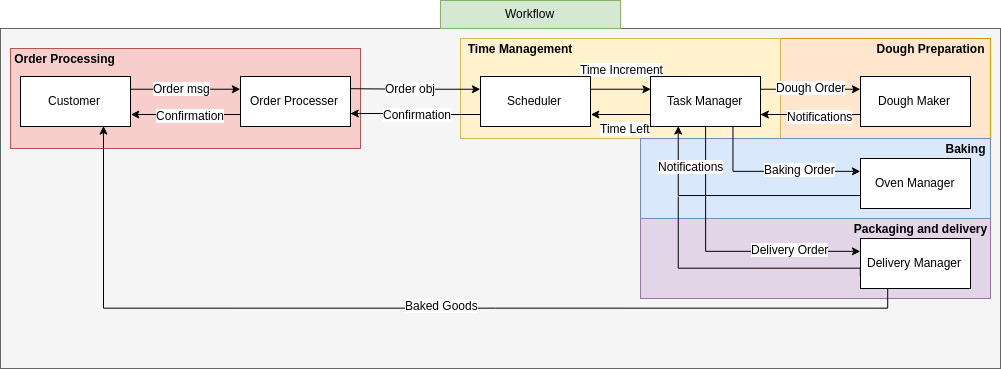
\includegraphics[scale=0.4]{img/architecture-pipeline.png}
		\caption{Workflow of the architecture.}
		\label{fig: WF}
	\end{figure}
	
	\subsection{Workflow description}
	The way our workflow was designed, as it can be appreciated in Figure \ref{fig: WF}, englobes all the required stages, such as order processing, dough preparation, baking, packaging, and delivery. As it can be appreciated in the detailed description below we decided not to create proofer, cooling racks, loading bays, nor mailboxes, but treat those process as behaviors from our defined agents.
	
	The following subsections were designed to explain in more details the whole process from receiving an order to delivering the requested products.
	 
	\subsubsection{Receiving Orders}
	
	The Customer creates an order specifying the desired products and the date of deliver, for instance: on day, 07.11 of 50 croissants, 30 donuts, 20 brezel, and 10 berliners, for 08.11. The order message is sent to the Order Processer. 
	
	The Order Processer reads the order message information and creates an order object. 
	
	The Order Processer sends the order object to the Scheduler, as it is the one that is keeping track of the current schedule of the bakery.
	
	The Scheduler receives the order object and checks in the calendar object if there is an empty spot for the delivery day of the new order and confirms/rejects the order depending on answer of that evaluation condition. Then, it sends a confirmation message to the Order Processer so that it can confirm the customer that the order can be processed. 
	
	\subsubsection{Production}
	
	The Scheduler creates a Task Manager for each order that needs to be produced on the current date, passing the order object as an attribute. 
	
	The task manager creates one baked good object per product in the order. 
	
	The task manager selects the product type with the biggest quantity and creates the respective dough order, and sends it to the Dough Maker. This is repeated for all the product types in the order.
	
	The dough maker verifies if it can produce the needed dough volume based on the availability of kneading machines. If not, it stores the dough order in a queue. 
	
	Based on the volume in the dough order, it determines the number of kneading machines needed.
	
	Once the kneading machine timer is over, the dough is set to rest for the specific resting time for that product type. 
	
	The dough maker repeats the process of loading the kneading machines, kneading the dough, and putting the dough to rest for each dough order in the queue.
	
	Once the dough resting time is over, a notification message is sent to the Task Manager.
	
	Once a notification from the Dough Maker is received, the Task Manager creates a baking order and sends it to the Oven Manager. Note that a baking order is created per dough order, which is indeed created per product type.
	
	The Oven Manager receives the baking order and computes the number of trays that is going to require. Checks the current temperature of each tray and, if needed, heats it up until it reaches the baking temperature. 
	
	Once the tray has reached the baking temperature, it gets filled out, and the baking process starts. 
	
	Once the baking time has finished, a notification is sent to the Task Manager to confirm that the bread is ready to start the cool down process. 
	
	The task manager waits until the temperature of the products reach the boxing temperature, and once all the products in the original order have been baked, and reached the boxing temperature it sends a delivery order to the Delivery Manager. The Delivery Manager receives the baked products and store them in a box, making sure that each of the box does not contains products of different types.
	
	The Delivery Manager fills up a truck with the boxes of products. Using the street network map, it travels to the customer destination and delivers the requested products. 
	
	Once the order has been delivered to the customer, the Delivery Manager notifies the Task Manager. 
	
	The Task Manager agent dies once the whole order process has been finished. 
	
	\subsubsection{Time updates}
	Throughout the process the Scheduler communicates with the Task Manager to keep track of the order and keep the calendar up to date. 
	
	At the moment of the creation of the Task Manager, it reports the time left of the current order, and, throughout the process, reports the time left at every stage, i.e. when the Dough Maker finishes the dough, the Oven Manager, finishes baking, and when the order is being delivered. 
	
	Once the Scheduler receives a time left message from every Task Manager, it sends a time increment message to all the Task Managers to update the current time of all of them. 	
	
	\newpage
	
	 \section{Agents}
	 
	 \begin{figure}[h!]
	 	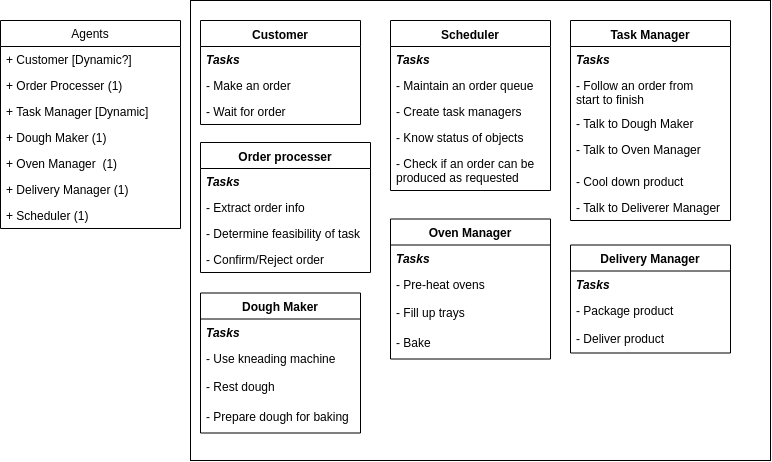
\includegraphics[scale=0.5]{img/architecture-Agents.png}
	 	\caption{Agents that conforms the system.}
	 	\label{fig: Ag}
	 \end{figure}
	 
	 \subsection{Agents descriptions}
	 
	 The Figure \ref{fig: Ag} helps to illustrate all the agents that play a role in our architecture. Additionally, it is shown which agents are dynamic, and which are static having a fixed number of those agents at the moment of launching the system. Lastly, it is also displayed the set of tasks is agent is going to performed.
	 
	 \begin{itemize}
	 	\item{\textbf{Customer:} \\
	 		- \textit{Description}:\\
	 		Agent created whenever we want to create an order to the bakery. \\
	 		- \textit{Behaviors:} \\
	 		1. Make an order (One-shot).}
	 	
		 \item{\textbf{Order Processer:} \\
		 	- \textit{Description}:\\
		 	Static agent that interacts with Customer agent to receives an order. \\
		 	- \textit{Behaviors:} \\
		 	1. Receive order (One-shot). \\
		 	2. Confirm/Reject order (One-shot).}
		 
		 \item{\textbf{Scheduler:} \\
		 	- \textit{Description}:\\
		 	Static agent created to manage time and calendar of the bakery. \\
		 	- \textit{Behaviors:} \\
		 	1. Query calendar (One-shot).\\
		 	2. Update calendar (One-shot).\\
		 	3. Create Task Manager (One-shot).\\
		 	4. Updates global time (One-shot).}
		 
		 \item{\textbf{Task Manager:} \\
		 	- \textit{Description}:\\
		 	Static created to manage an order. \\
		 	- \textit{Behaviors:} \\
		 	1. Update own time (One-shot).\\
		 	2. Produce Order (Generic).\\
		 	3. Create dough order (One-shot).\\
		 	4. Create baking order (One-shot).\\
		 	5. Create delivery order (One-shot).\\
		 	6. Cool down product (Generic).\\
		 	7. Report time left (One-shot). \\
		 	8. Process notification (One-shot).}
		 
		 \item{\textbf{Dough Maker:} \\
		 	- \textit{Description}:\\
		 	Static agent created to prepare the dough. \\
		 	- \textit{Behaviors:} \\
		 	1. Process dough order (One-shot).\\
		 	2. Make dough (Generic).\\
		 	3. Rest dough (Generic).\\
		 	4. Send notification (One-shot).}
		 
		 \item{\textbf{Oven Manager:} \\
		 	- \textit{Description}:\\
		 	Static agent created to bake bread. \\
		 	- \textit{Behaviors:} \\
		 	1. Process baking order (One-shot).\\
		 	2. Pre-heat trays (Generic).\\
		 	3. Bake bread (Generic).\\
		 	4. Send notification (One-shot).}
		 
		 \item{\textbf{Delivery Manager:} \\
		 	- \textit{Description}:\\
		 	Static agent created to delivery products. \\
		 	- \textit{Behaviors:} \\
		 	1. Process deliver order (One-shot).\\
		 	2. Box product (One-shot).\\
		 	3. Load truck (One-shot).\\
		 	4. Send notification (One-shot).}
	 \end{itemize}
	 \newpage
	 \section{Objects}
	 
	 \begin{figure}[h!]
	 	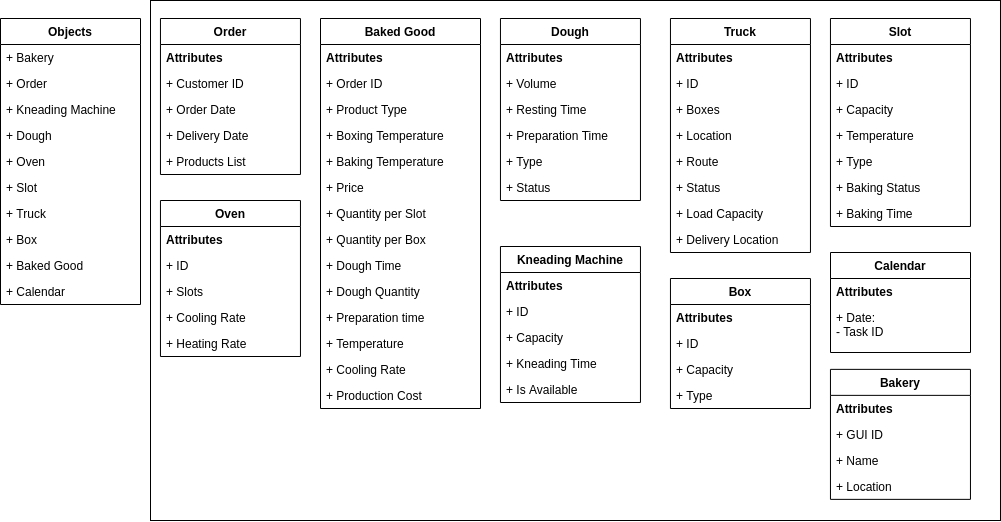
\includegraphics[scale=0.4]{img/architecture-Objects.png}
	 	\caption{Objects used in the system.}
	 	\label{fig: ob}
	 \end{figure}
	
	The Figure \ref{fig: ob} helps to illustrate the different objects that constitute our architecture, as well as the different attributes that are assigned to each of the objects. 
\end{document}